\textbf{\textit{``Whereof one cannot speak, thereof one must be silent.''}}

Ludwig Wittgenstein (1889 – 1951)

\chapter{Results}
Of over seven million incident reports, 7273 were classified by NPSA staff as belonging to ``Infrastructure (including staffing, facilities, environment)'' (incident category level 1) and ``IT / telecommunications failure / overload'' (incident category level 2) categories. These were selected to form the ``computer problem'' extract (since it was felt that computer problems would fall under this classification category).

\section{Descriptive statistics}

\subsection{Data quality}
\label{dataqualityresults}

The NRLS ``computer problem'' extract contains 7273 rows of data. Each row represents a clinical incident report. Each column represents one of 32 fields (See tables \ref{tab:field_names1} and \ref{tab:field_names2}) which are extracted from the incident report form and cleaned to remove sensitive data by the NRLS. The dataset contained 159 duplicates (Table \ref{tab:duplicates}) which were removed before further analysis was carried out. The completeness of fields varied considerably and some fields were derived entirely from other fields, for example, the age range field is populated by the patient age field. 

The median number of words in the free text incident description field (IN07) was 35 and the range spanned 1-730, this was a mandatory field (see section \ref{dataqualitymethod}).


\begin{table}[htbp]\centering
\begin{tabular}{lr}
\toprule
\textbf{Is the description of the incident a duplicate?} & {} \\
\midrule
False &	7114 \\
True  &	159 \\
\bottomrule
\end{tabular}
\caption{Incident reports in the computer problem dataset with identical incident descriptions (duplicates)}
\label{tab:duplicates}
\end{table}

\begin{table}[htbp]\centering
\begin{tabular}{lr}
\toprule
\textbf{Spelling variant} & {\textbf{N}} \\
\midrule
Anaes	& 1 \\
Anaesetic & 	1 \\
anaeshthetist &	1 \\
anaestetist & 1 \\
anaesth	& 1 \\
Anaesthatised &	1 \\
Anaesthatist &	1 \\
anaesthesia & 1 \\
ANAESTHESIST &	1 \\
anaesthetic &	39 \\
Anaesthetic &	11 \\
ANAESTHETIC &	3 \\
anaesthetics &	4 \\
Anaesthetics &	2 \\
anaesthetied &	1 \\
anaesthetise &	1 \\
anaesthetised &	5 \\
anaesthetising & 1 \\
ANAESTHETIST &	6 \\
anaesthetist & 54 \\
Anaesthetist & 21\\
anaesthetist4 &	1\\
anaesthetists & 3\\
anaesthtic & 1\\
anaethestised &	1\\
anaethetised & 1 \\
anaethetist &	3\\
Anaethetist &	1\\
anaethetists &	1\\
\end{tabular}
\label{tab:spelling variants of anethtist}
\caption{There were 31 spelling variants of anaethetist and related terms in the computer problem data set. Acronyms were also commonplace. Without reconciliation spelling variants and acronyms can be detrimental to machine learning tasks such as clustering and classifying.}
\end{table}



\begin{table}[htbp]\centering
\begin{tabular}{lr}
\toprule
\textbf{Field name} & \textbf{Field completeness{(\%)}}\\
\midrule
Unique Incident Id & 100.0 \\
Age At Time Of Incident	Date & 30.0 \\
Incident Received By Npsa & 100.0\\	
Type Of Device & 6.0 \\
Patent Age At Time Of Incident & 30.0 \\
Date Record Exported To Nrls & 100.0\\
Date Of Incident & 99.9 \\
Location (lvl1) & 100.0 \\
Location (lvl2) & 99.7 \\
Location (lvl3) & 55.6 \\
Location - Free Text & 7.5 \\
Incident Category - Lvl1 & 100.0 \\
Incident Category - Lvl2 & 100.0 \\
Incident Category - Free Text & 0.0 \\
Free Text Description Of What Happened & 100.0\\
\bottomrule
\end{tabular}
\caption{Field names in the dataset and percentage completeness for the computer problem data set. Percentage field completeness is calculated by dividing the number of non-blank fields for a given field name by the number of incident reports, after removing duplicates, and multiplying by 100.}
\label{tab:field_names1}
\end{table}


\begin{table}[htbp]\centering
\begin{tabular}{lr}
\toprule
\textbf{Field name} & \textbf{Field completeness{(\%)}}\\
\midrule
Actions Preventing Re-occurrence & 38.0 \\
Apparent Causes & 21.5 \\
Med Process & 1.6 \\
Med Error Category & 1.5 \\
Approved Name (drug 1) & 0.1 \\
Proprietary Name (drug 1) & 0.0	\\
Patient Age Range & 30.3	\\
Patient Sex & 55.5	\\
Specialty - Lvl 1 & 100.0 \\
Specialty - Lvl 2 & 63.3	\\
Speciality - Free Text & 18.8\\	
Degree Of Harm (severity) & 100.0\\
Paediatric Care & 29.9 \\
Source Of Notification & 100.0\\
Care Setting Of Occurrence & 100.0 \\
Reason Exclusion & 0.0\\
\bottomrule
\end{tabular}
\caption{Field names in the dataset and percentage completeness. Percentage field completeness is calculated by dividing the number of non-blank fields for a given field name by the number of incident reports, after removing duplicates, and multiplying by 100.}
\label{tab:field_names2}
\end{table}

\subsection{Sample breakdown}
The NRLS incident reporting form has 5 categories of patient harm: 

\begin{enumerate}
 \item no harm
 \item low harm
 \item moderate harm
 \item severe harm
 \item death
\end{enumerate}

The computer problem sample is similar to the totality of incident reports submitted to the NRLS in that no harm and low harm incidents are reported more frequently than more serious incidents such as severe harm and death. See tables \ref{tab:harm1}, \ref{tab:degreeharm}, \ref{tab:specialty}, and \ref{tab:location} for details. 


\begin{table}[htbp]\centering
\begin{tabular}{l p{10cm}}
\toprule
\textbf{Harm} & \textbf{NPSA definition} \\
\midrule
No Harm & A situation where no harm occurred: either a ‘prevented patient safety incident’ or a ‘no harm patient safety incident’. \\
Low & Any unexpected or unintended incident which required extra observation or minor treatment and caused minimal harm, to one or more persons. \\
Moderate & Any unexpected or unintended incident which resulted in further treatment, possible surgical intervention, cancelling of treatment or transfer to another area and which caused short-term harm, to one or more persons. \\
Severe & Any unexpected or unintended incident which caused permanent or long-term harm, to one or more persons. \\
Death & Any unexpected or unintended incident which caused the death of one or more persons.\\
\bottomrule
\end{tabular}
\label{tab:harm1}
\caption{NPSA classification of degree of harm caused by incidents.}
\end{table}



\begin{table}[htbp]\centering
\begin{tabular}{lr}
\toprule
\textbf{What was the degree of harm?} & {\textbf{N}} \\
\midrule

No Harm & 5982 \\
Low & 792 \\
Moderate & 268 \\
Severe	& 65 \\
Death & 7 \\


\bottomrule
\end{tabular}
\label{tab:degreeharm}
\caption{Degree of harm caused by incidents relating to computer problems.}
\end{table}


\begin{table}[htbp]\centering
\begin{tabular}{lr}
\toprule
\textbf{Specialty} & {\textbf{N}} \\
\midrule
Medical specialties & 1104 \\
Diagnostic services &	1039\\
Not applicable &	995\\
Obstetrics and gynaecology &	695\\
Surgical specialities &	673\\
Other	& 600\\
Unknown	& 526\\
Primary care / Community	& 508\\
Accident and Emergency &	415\\
Other specialities &	137\\
Mental health &	123\\
PTS (Patient Transport Service) &	98\\
Learning disabilities & 78\\
Anaesthesia Pain Management and Critical Care & 62\\
Dentistry - General and Community &	60\\
Children’s Specialities	& 1\\
\bottomrule
\end{tabular}
\label{tab:specialty}
\caption{Speciality involved in computer incidents, based on level one data.}
\end{table}


\begin{table}[htbp]\centering
\begin{tabular}{lr}
\toprule
\textbf{Speciality} & {\textbf{N}} \\
\midrule
Acute / general hospital &	5054\\
Ambulance service &	121\\
Community and general dental service & 34\\
Community nursing, medical and therapy service (incl. community hospital) &	1614\\
General practice &	92\\
Learning disabilities service &	17\\
Mental health service	& 182\\
\bottomrule
\end{tabular}
\label{tab:location}
\caption{Location of the computer incidents, based on care setting data.}
\end{table}


\section{Data exploration}
\label{themesresults}
Exploring the data with Grep, Apache and Solr (see section \ref{themesmethod}) confirmed the prescence of two major themes suspected to be present, namely, poor systems reliability and problems not being fixed promptly. 


\subsection{Grep}

Greps for terms the author thought might be interesting such as ``crash'', ``freeze'', ``locked'', and ``unable'', returned many records and gave a flavour of how healthcare professionals report computer problems.

\begin{figure}[htp]
\centering
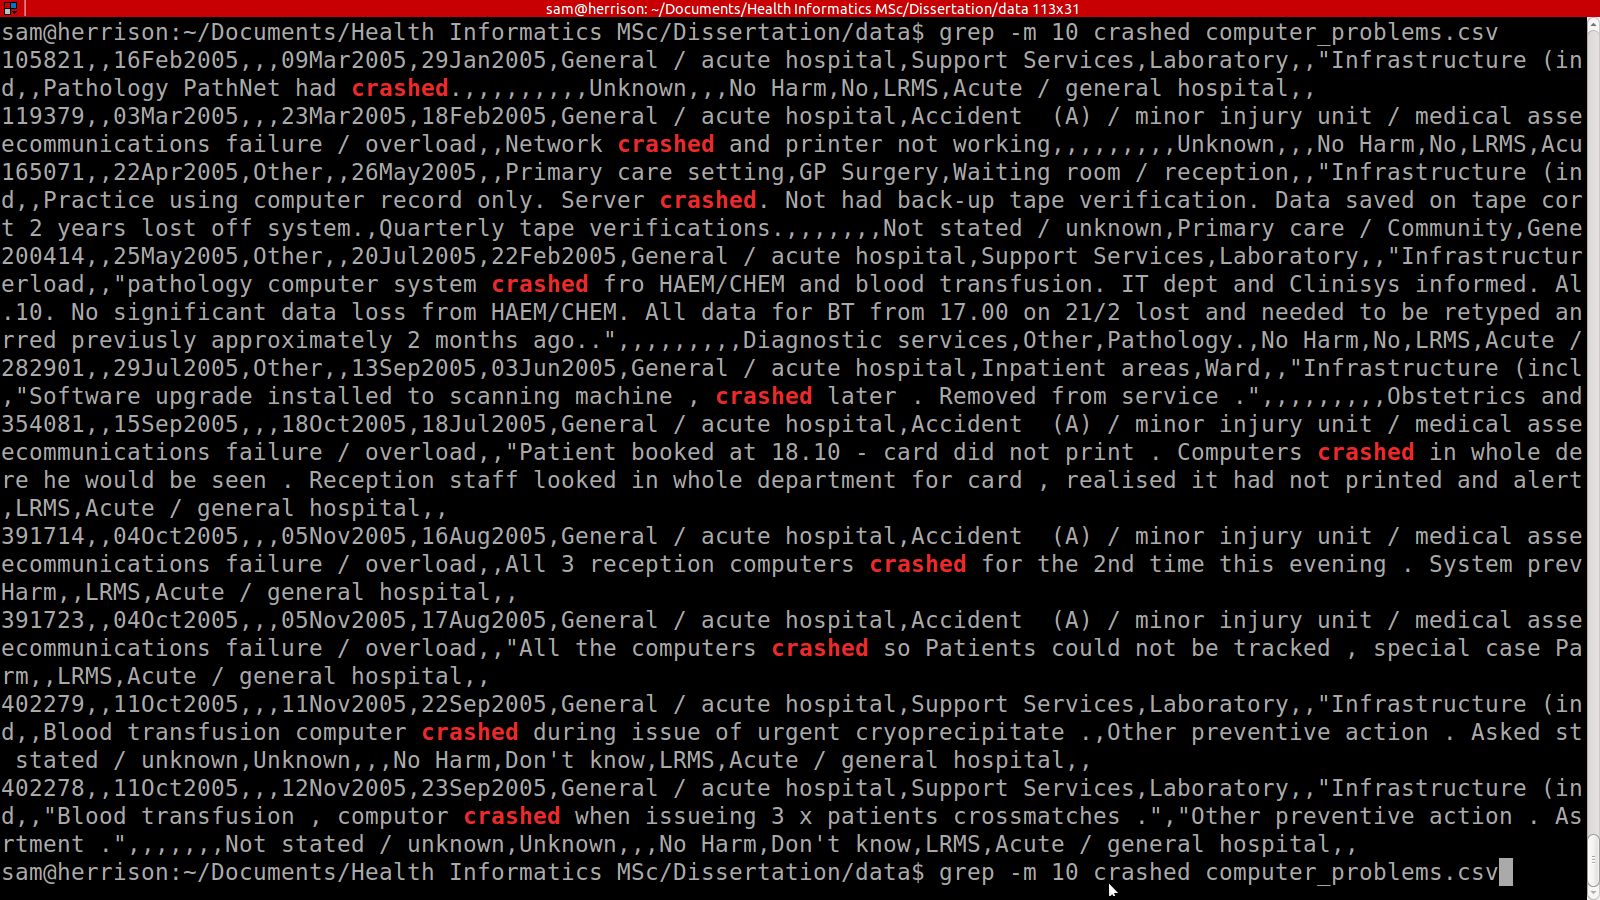
\includegraphics[width=15cm,height=10cm]{figs/grepcrashed10.png}
\caption{Grep results for search on term ``crash''.}\label{fig:bugsa}
\end{figure}

\begin{figure}[htp]
\centering
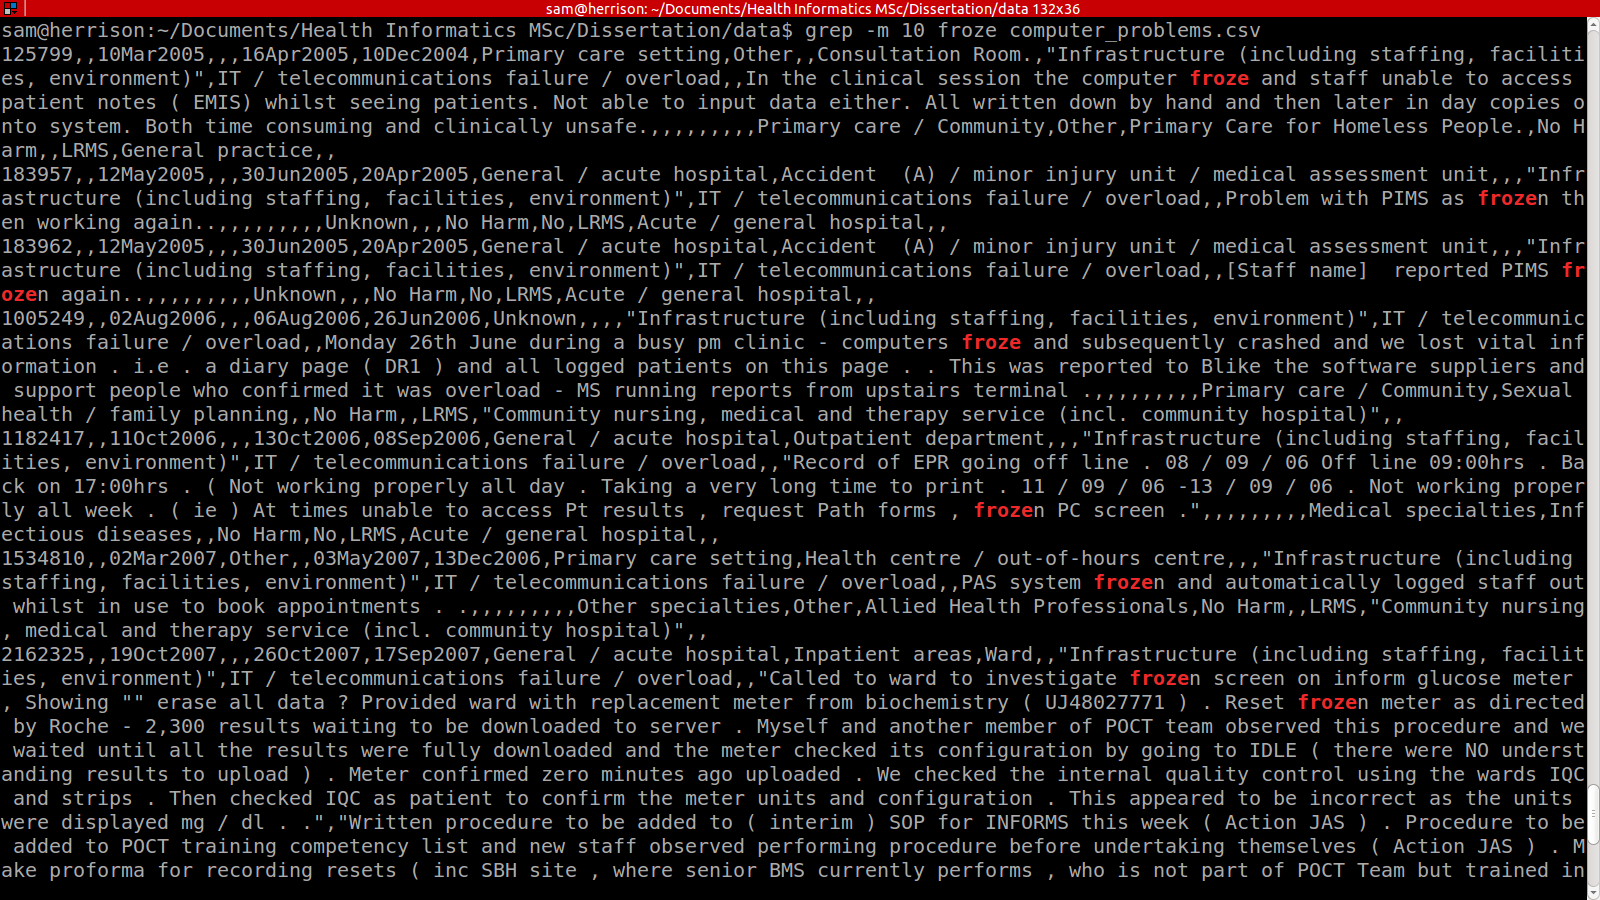
\includegraphics[width=15cm,height=10cm]{figs/grepfroze10.png}
\caption{Grep results for search on term ``freeze''.}\label{fig:bugsb}
\end{figure}

\begin{figure}[htp]
\centering
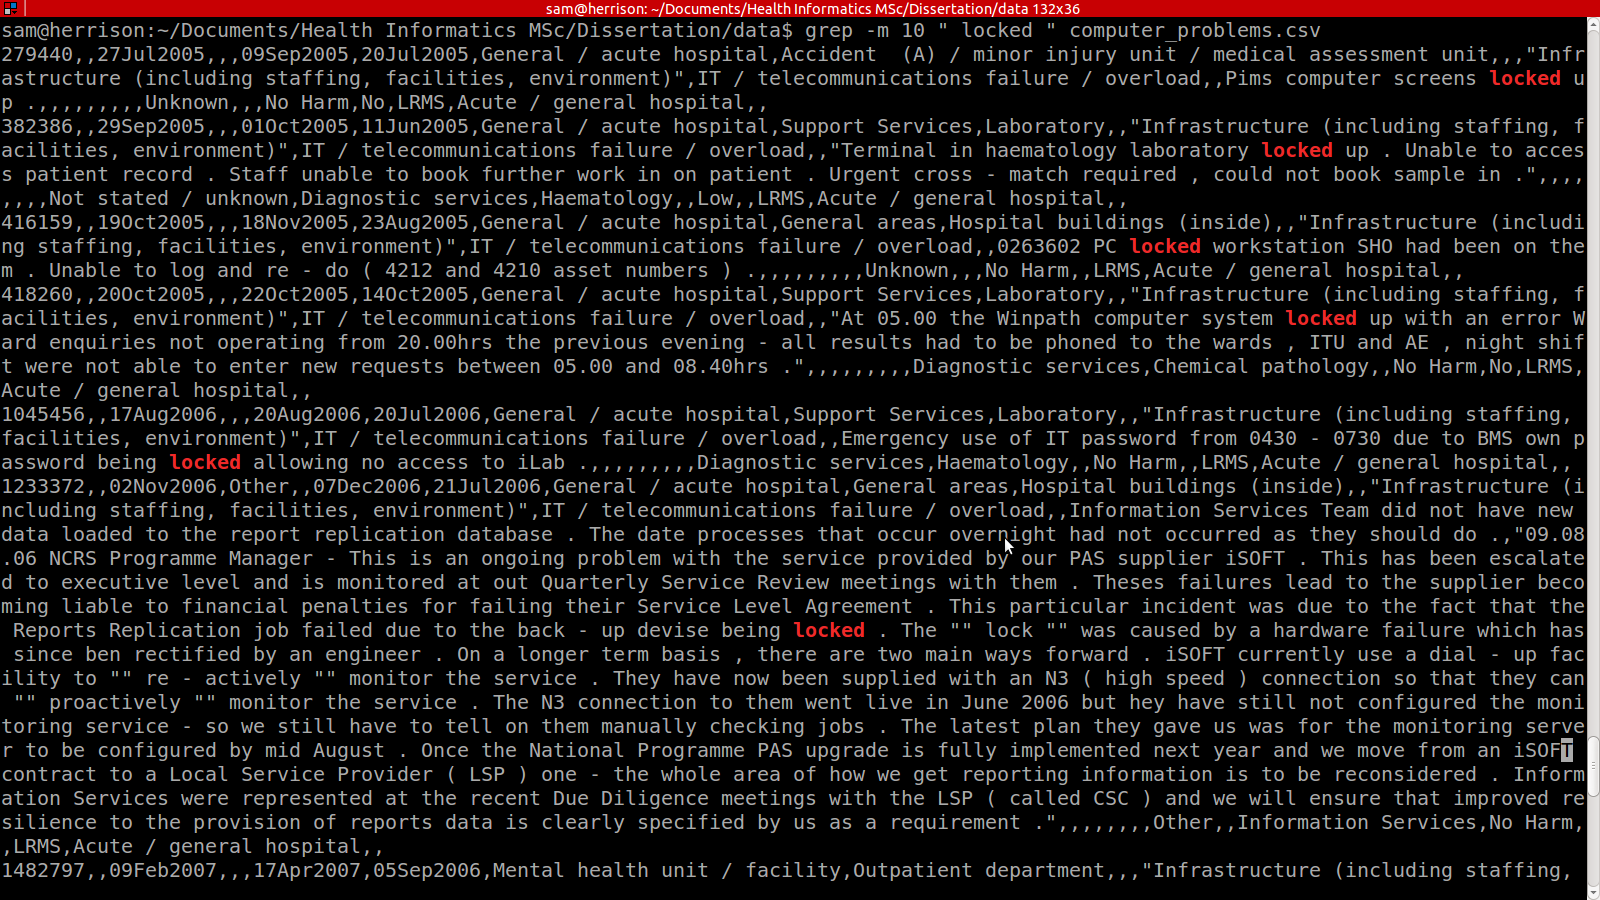
\includegraphics[width=15cm,height=10cm]{figs/greplocked10.png}
\caption{Grep results for search on term ``locked''.}\label{fig:bugsc}
\end{figure}

\begin{figure}[htp]
\centering
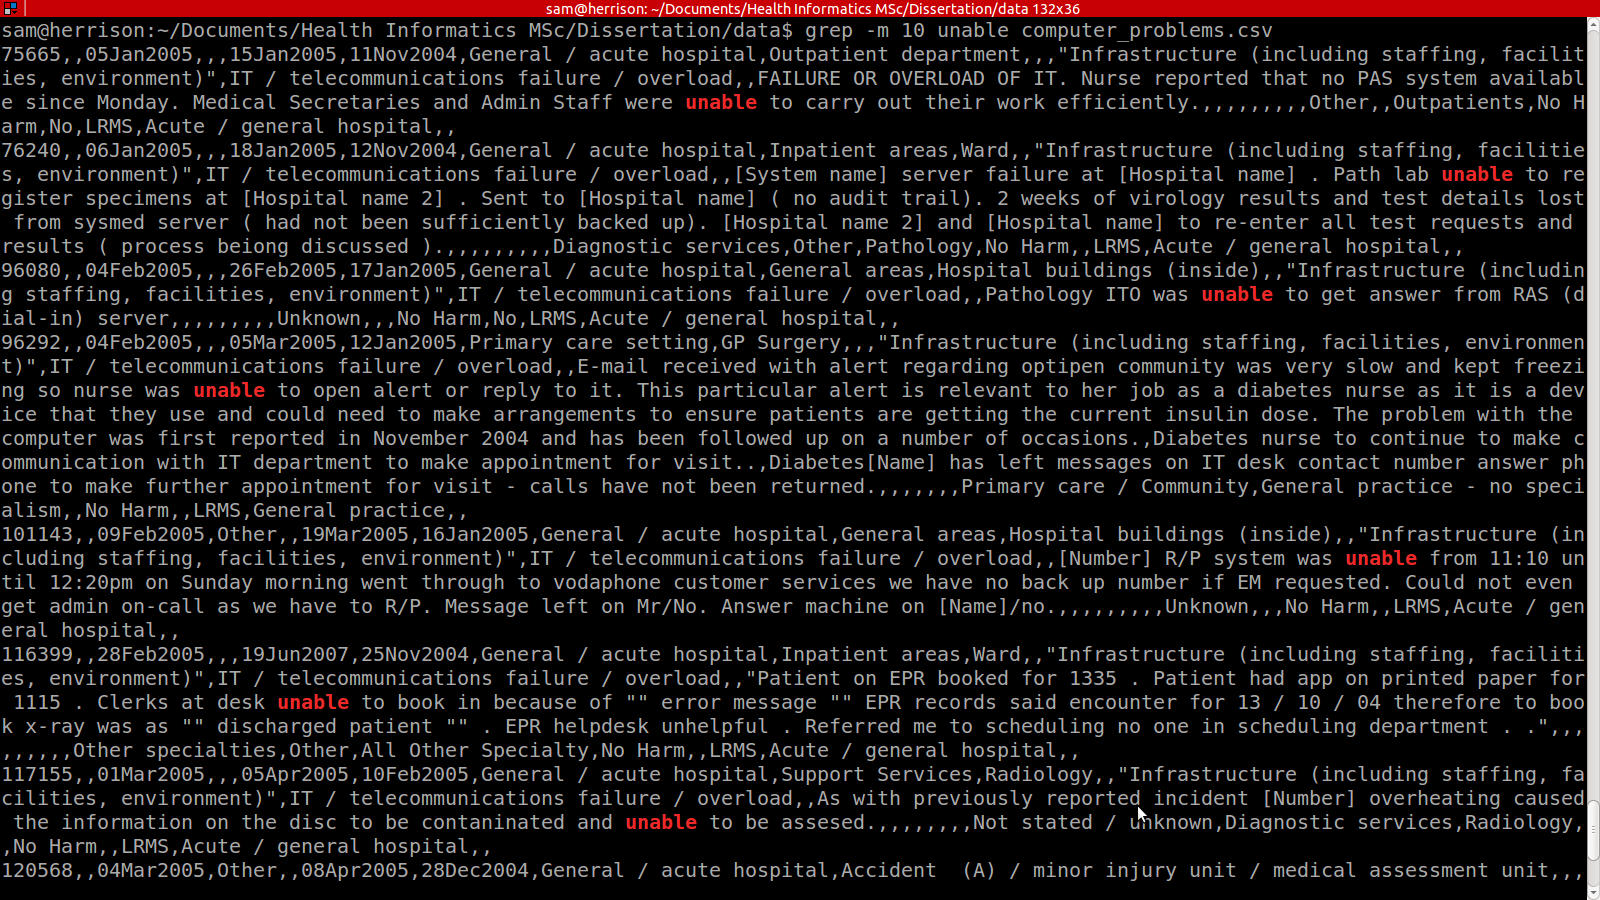
\includegraphics[width=15cm,height=10cm]{figs/grepunable10.png}
\caption{Grep results for search on term ``unable''.}\label{fig:bugsd}
\end{figure}



\subsection{Solr}

\paragraph{Poor system reliability}

Poor system reliability was identified as a theme and terms associated with poor reliability such as ``crashed'' were combined in a search using Solr.

\begin{figure}[htp]
\centering
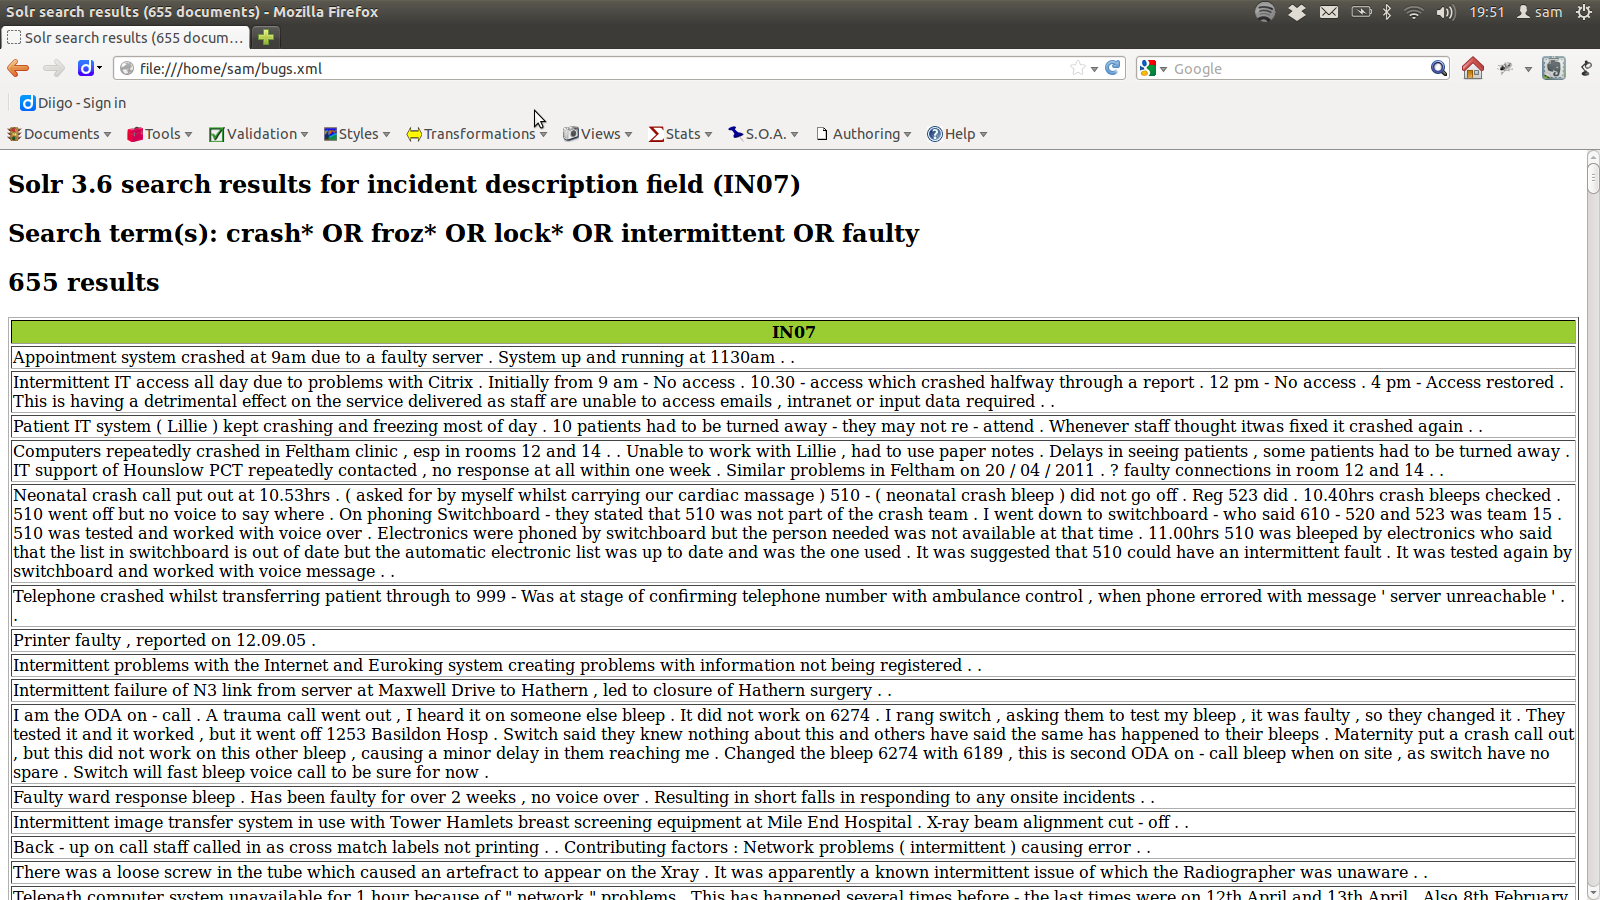
\includegraphics[width=15cm,height=10cm]{figs/bugs.png}
\caption{Search results for search of the computer problems data set for terms associated with poor system reliability.}\label{fig:bugs}
\end{figure}


\paragraph{Problems not fixed promptly}


\begin{figure}[htp]
\centering
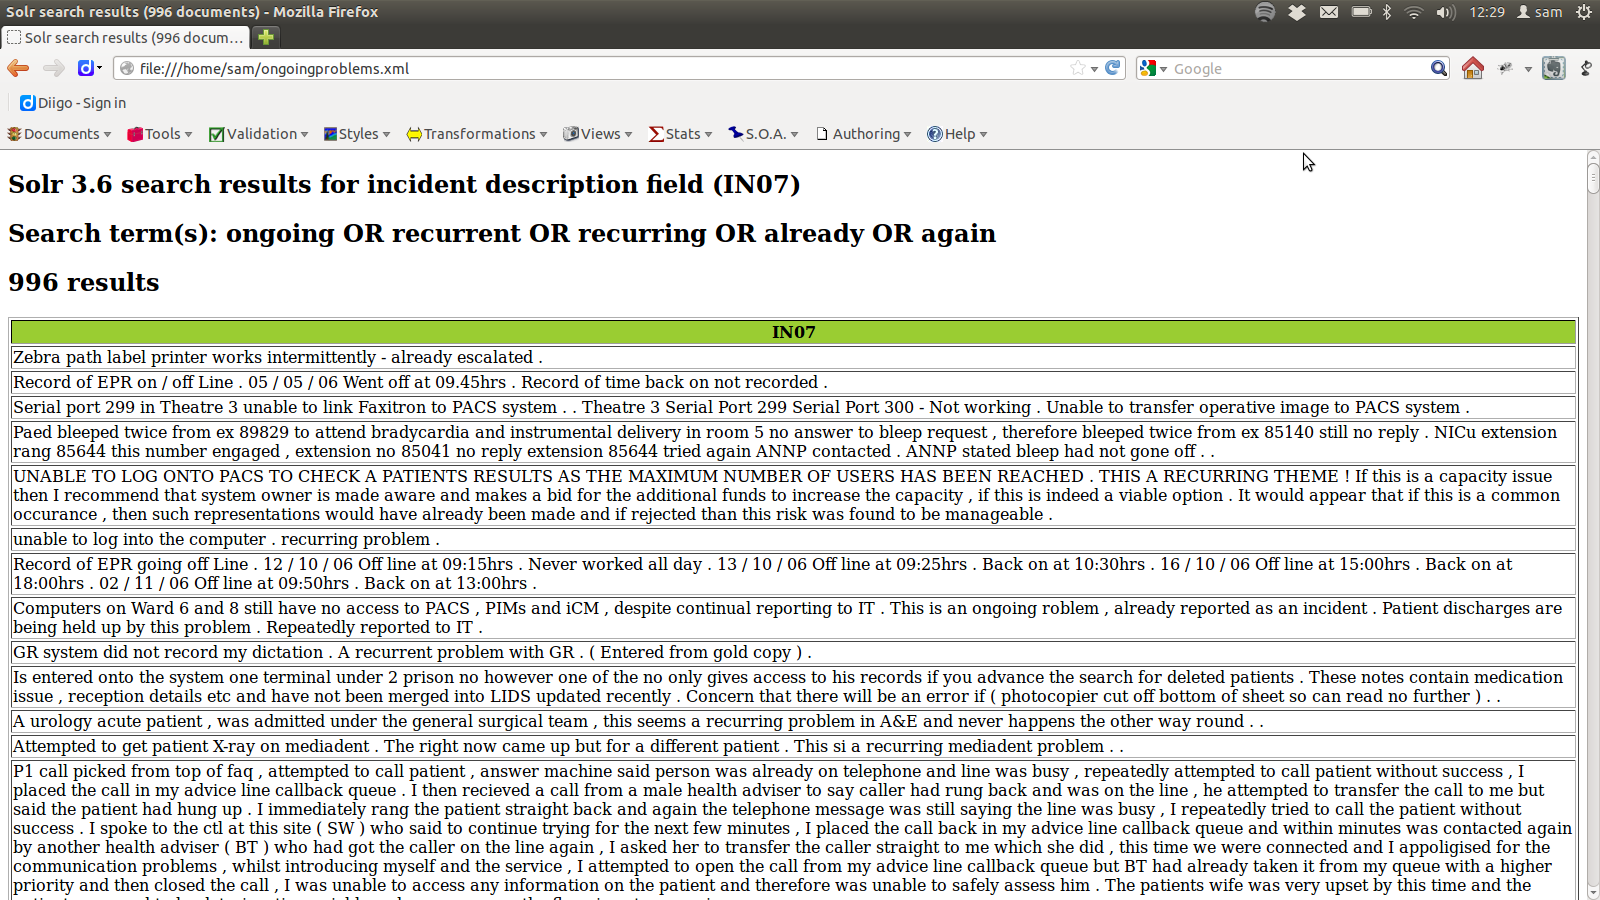
\includegraphics[width=15cm,height=10cm]{figs/ongoingproblems.png}
\caption{Searching the computer problems dataset for terms which might indicate an ongoing problem such as ``ongoing OR recurrent OR recurring OR already OR again'' yielded 996 results.}\label{fig:ongoingproblems}
\end{figure}

Example incident reports identified by Solr using search on terms which might indicate ongoing computer problems.
\begin{itemize}
 \item ``Yet again 400 + results , some a year old , have appeared today for signing off . This is a significant risk which has been highlighted repeatedly and I am not aware that any action has been taken / or even that a clear explanation has been given for why it occurs . ( Examples of 4 sample patients listed on form . ) .''
 \item ``Computerised ' Carevue' system for charting vital sighs and ventilation on Nicu and Picu freezing over past 24hrs . ICT phoned x2 and team in Vienna investigating . Was rebooted overnight . At 06.15 the carevue system again froze , this time completely , not allowing any entering or viewing of screens . This has an impact on patient safety as the day staff cannot review the patients and accuratly assess their clinical stability and plan treatment accordinglyly . Also , 2 new patients to NICU overnight , who clinical information cannot be accessed . .''
\end{itemize}


\subsection{NLTK}
\label{lexicalanalysisresults}

Basic lexial analysis was carried out using NLTK (see section \ref{lexicalanalysismethod}). This proved most useful for drilling down and exploring snippets relating to a theme identified by the lingo clustering algorithm, namely of users reporting being unable to do things because of computer system failure (see section \ref{unabletosnippetsresults}).


\subsubsection{Basic lexical statistics}
There were 408657 words in the text. 14018 words formed the vocabulary. The lexical diversity (number of words in text/vocabulary) was 29 (see section \ref{lexicalanalysismethod}).


\subsubsection{Collocations}

A collocation is a sequence of words that occur together unusually often. Thus, ``red wine'' is a collocation, whereas ``the wine'' is not. Collocations are resistant to substitution, for example, ``maroon wine'' would sound very odd. They tend to be specific to a given text and so can convey useful information.\cite{Bird2009}

Collocations identified in ``computer problem'' extract were:

\begin{itemize}
 \item Staff Name
 \item cardiac arrest
 \item computer system
 \item Health Advisor
 \item warm transfer
 \item staff member
 \item Contributing factors
 \item labour ward
 \item switch board
 \item health advisor
 \item call back
 \item Staff member
 \item blood results
 \item NHS Direct
 \item several times
 \item help desk
 \item ambulance control
 \item File Closed
 \item ambulance service
 \item Staff name
\end{itemize}

The top 10 \gls{point wise mutual information} trigrams, filtering for (removing) those occurring less than 10 times, were: 

\begin{itemize}
 \item First Advice Queue
 \item Abbott Diagnostic where
 \item regarding poor connectivity
 \item ongoing issues regarding
 \item serial no C160045
 \item instrument serial no
 \item issues regarding poor
 \item contributing factors
 \item front sheet did
\end{itemize}

\begin{figure}[htp]
\centering
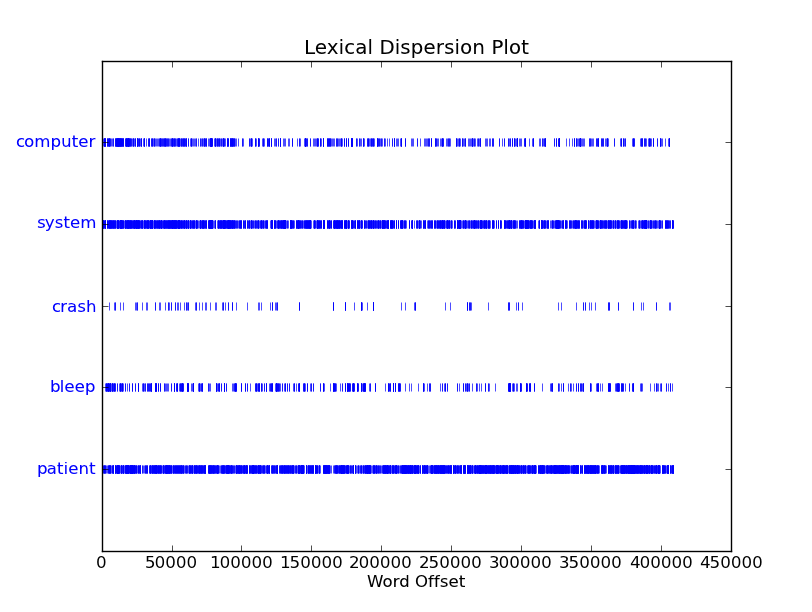
\includegraphics[width=15cm,height=10cm]{figs/lexicaldispersionplot.png}
\caption{Each stripe represents an instance of a word and each row represents the entire text. If present, trends in the frequency of the use of words over time can be visualized in this way (the incident descriptions forming the text have been time ordered).}\label{fig:lexicaldispersionplot}
\end{figure}


\begin{figure}[htp]
\centering
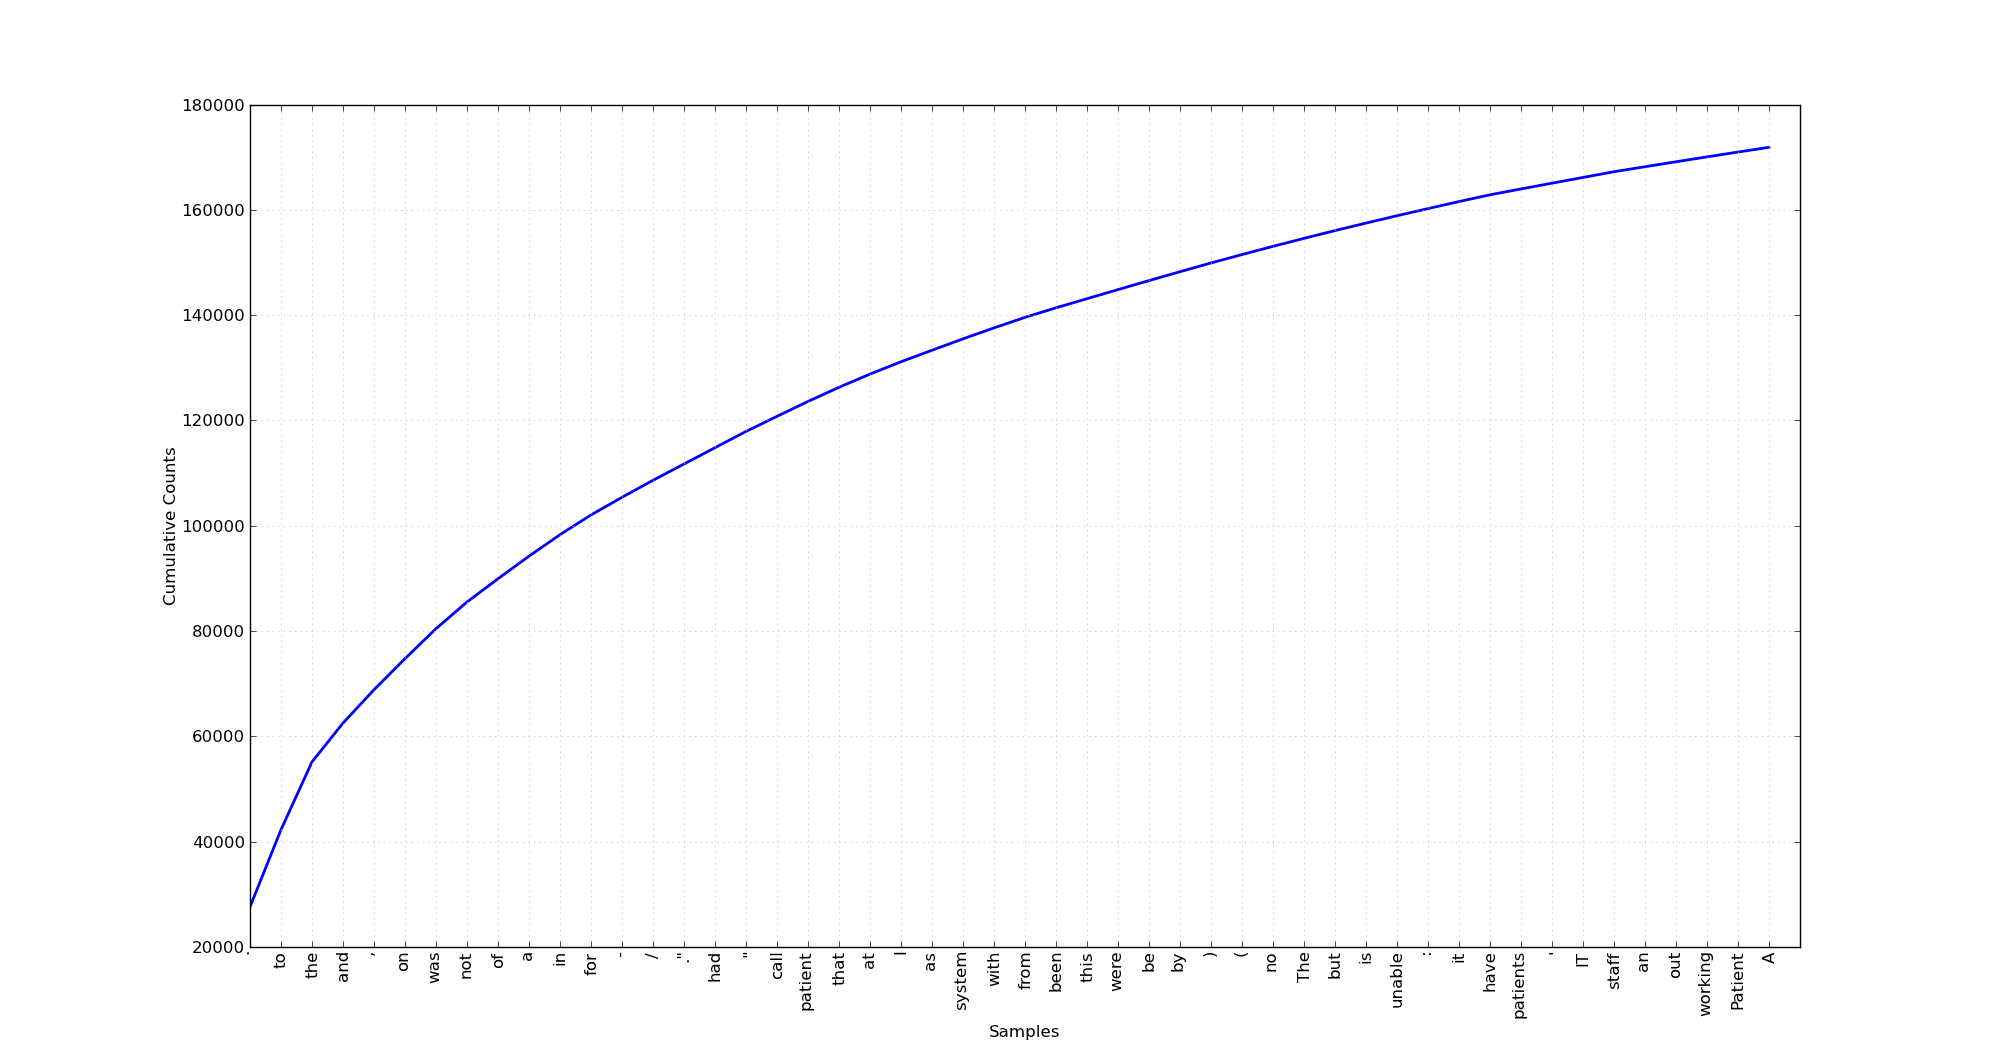
\includegraphics[width=15cm,height=10cm]{figs/cummulativedistribution.png}
\caption{Cumulative frequency plot for the 50 most frequently used words in incident reports about computer problems.}\label{fig:cumulativedistribution}
 \end{figure}



\subsubsection{Unable to snippets}
\label{unabletosnippetsresults}
A subset of poor system reliability was identified as to do with reporters being unable to perform particular tasks due to computer system failure using the lingo clustering algorithm. Using NLTK it was established that the words ``unable to'' were followed by another word in 1398 instances. 256 unique words made up these instances.

Top 10 words to follow the expression ``unable to'' in the data set:
\begin{pyverbatim}
 [('access', 318),
 ('contact', 108),
 ('get', 84),
 ('print', 71),
 ('log', 68),
 ('transfer', 48),
 ('use', 47),
 ('view', 47),
 ('be', 43),
 ('hear', 42)]
\end{pyverbatim}

\begin{figure}[htp]
\centering
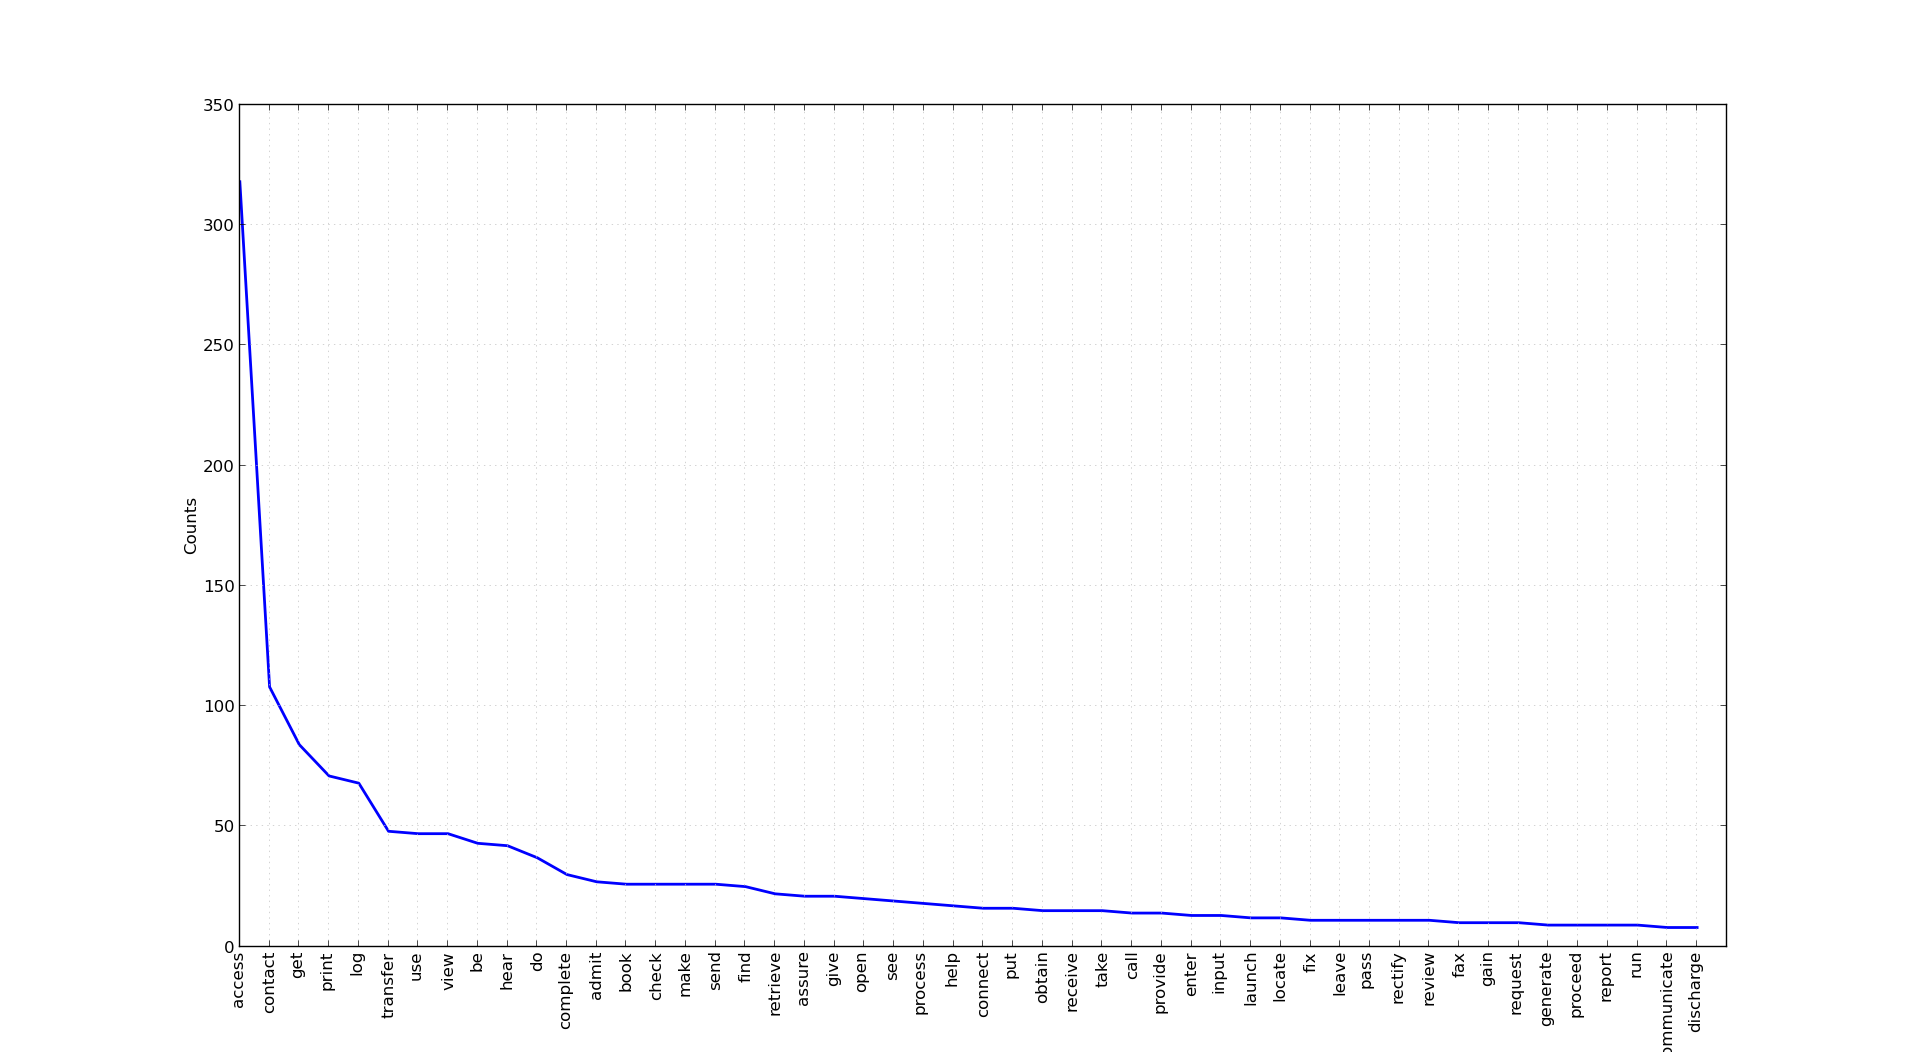
\includegraphics[width=15cm,height=10cm]{figs/unableto.png}
\caption{Frequency distribution plot of the 50 most common words to follow the words ``unable to'' in the text.}\label{fig:unableto}
\end{figure}

\subsubsection{Named entity recognition}

Parts of speech (POS) tagging was of very limited value in this case because the NPSA (usually) removes names of persons, companies, and locations, as part of their data cleaning.


\section{Lingo clustering algorithm}
\label{lingoresults}
Using the lingo clustering algorithm (see section \ref{lingomethod}) incidents are grouped without human supervision. The two most reliable discreet clusters identified were to do with bleep problems and being unable to access systems because of system failure (see section \ref{tab:lingo_topten_size}). Examples of incidents grouped under the bleep problem cluster selected to show the difficulty of the task are shown below (see section \ref{bleepproblemexamples}).

\begin{figure}[htp]
\centering
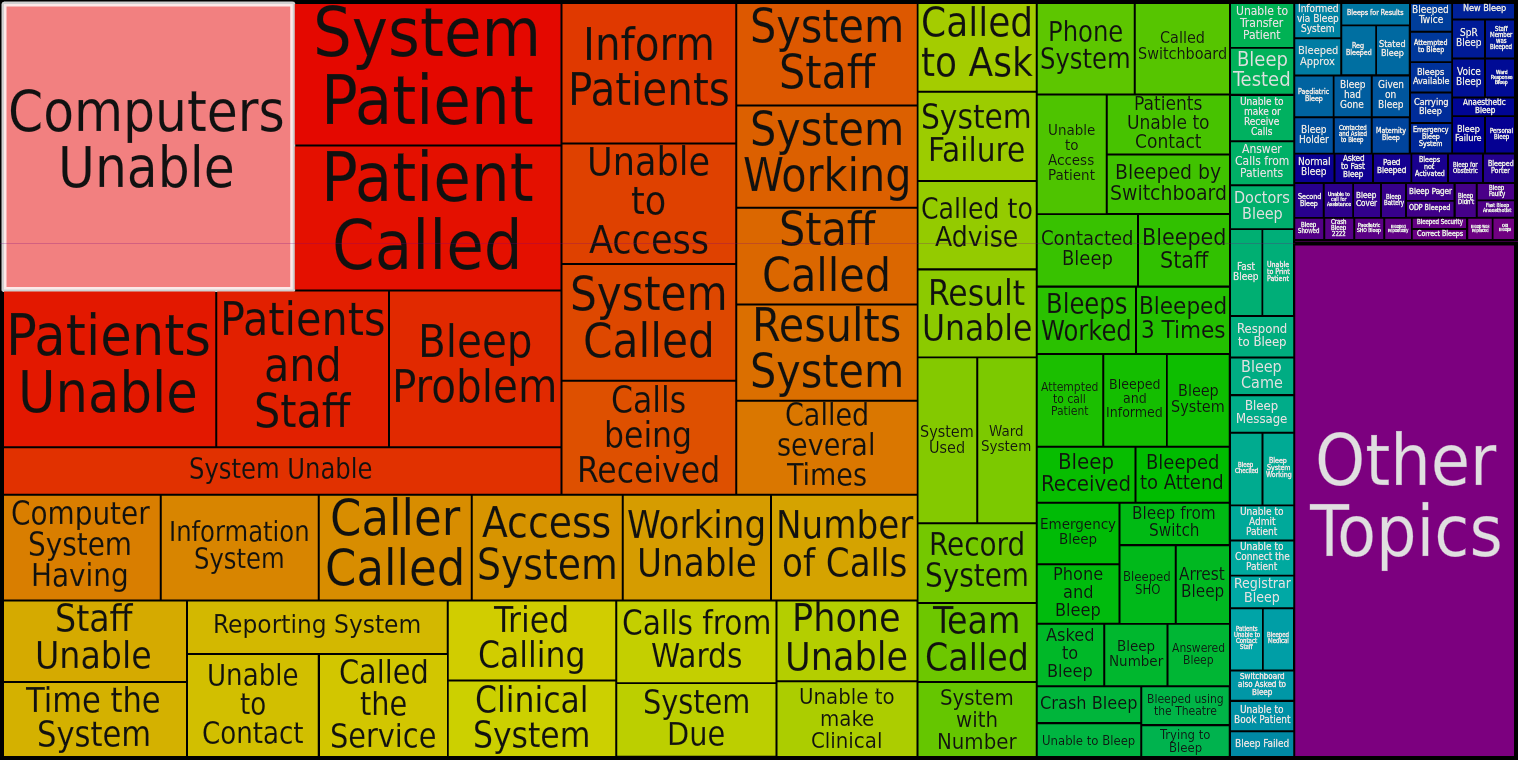
\includegraphics[width=15cm,height=10cm]{figs/lingoclustering.png}
\caption{Automatically generated clusters and labels with the lingo algorithm using the Carrot2 platform. Box size is proportional to the number of incidents within the cluster. Colour is arbitrary.}\label{fig:lingoclustering}
\end{figure}

\begin{figure}[htp]
\centering
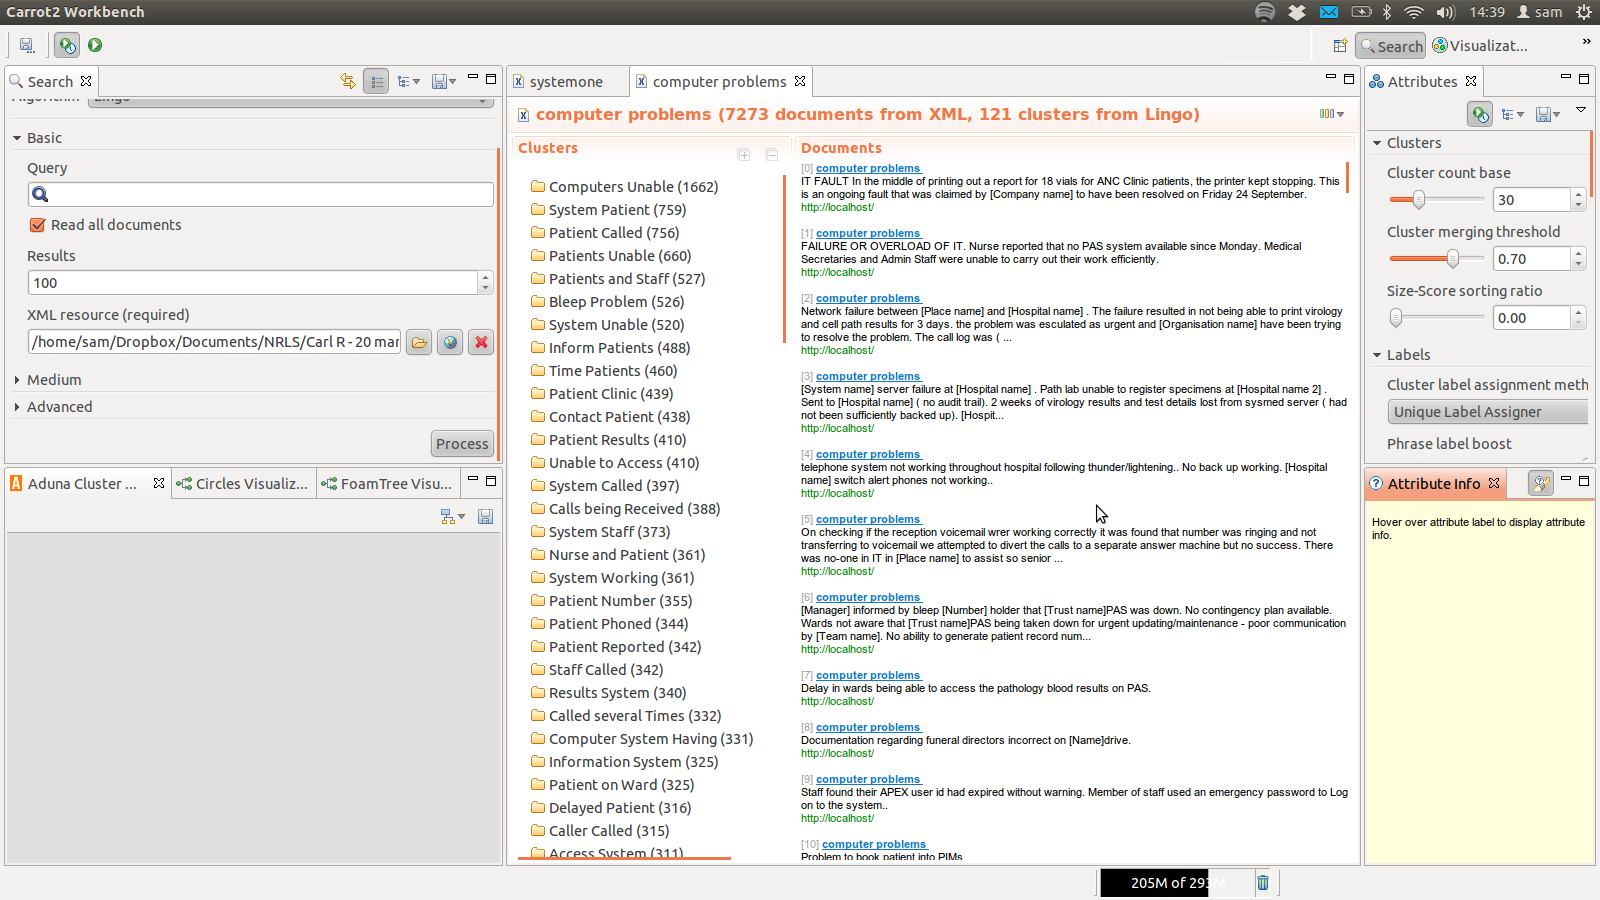
\includegraphics[width=15cm,height=10cm]{figs/clustering2.png}
\caption{Overview of the lingo clusters and setup screen.}\label{fig:lingoclustering2}
\end{figure}

\begin{figure}[htp]
\centering
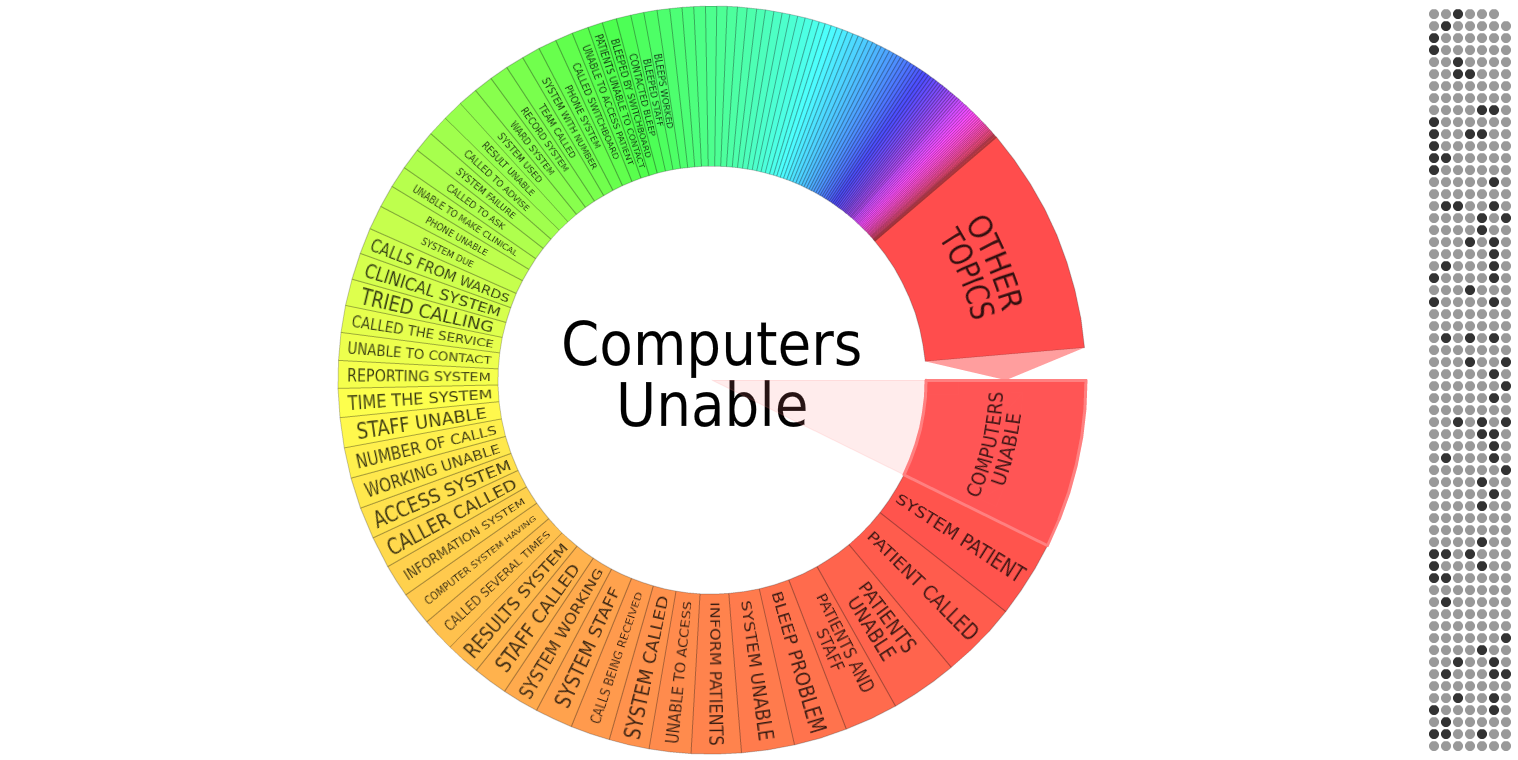
\includegraphics[width=15cm,height=10cm]{figs/lingoclusteringcircle.png}
\caption{Automatically generated clusters and labels with the lingo algorithm using the Carrot2 platform. Box size is proportional to the number of incidents within the cluster, circle visualisation. Colour is arbitrary.}\label{fig:lingoclusteringcircle}
\end{figure}


\newpage

\begin{table}[htbp]\centering
\begin{tabular}{lr}
\toprule
\textbf{Cluster label} & \textbf{Number of documents} \\
\midrule
Computers Unable & 1662 \\ 
System Patient & 759 \\ 
Patient Called & 756 \\ 
Patients Unable & 660 \\ 
Patients and Staff & 527 \\ 
Bleep Problem & 526 \\ 
System Unable & 520 \\ 
Inform Patients & 488 \\ 
Time Patients & 460 \\ 
Patient Clinic & 439 \\ 
\bottomrule
\end{tabular}
\label{tab:lingo_topten_size}
\caption{Automatically generated cluster labels for the ten largest clusters identified by the lingo algorithm}
\end{table}


\begin{table}[htbp]\centering
\begin{tabular}{lr}
\toprule
\textbf{Cluster label} & \textbf{Cluster reliability score} \\
\midrule
Bleep Problem & 21.8 \\ 
Unable to Access & 12.4 \\ 
System Staff & 11.0 \\ 
System Working & 10.3 \\ 
Calls being Received & 9.6 \\ 
Patients and Staff & 9.3 \\ 
Staff Called & 7.9 \\ 
Working Unable & 7.6 \\ 
Inform Patients & 7.4 \\ 
Called several Times & 7.4 \\ 
\bottomrule
\end{tabular}
\label{tab:lingo_topten_size}
\caption{Automatically generated cluster labels for the ten highest reliability scores identified by the lingo algorithm. The higher the reliability score the higher the reliability of the cluster content.}
\end{table}

\subsection{Bleep problems}
\label{bleepproblemexamples}

Bleep problems were identified as a large cluster with a high reliability score using lingo. However, these exerpts show that whlile some of the incidents identified are clearly to do with bleep problems others are not.

\begin{itemize}

 \item Bleep problem: ``ODP bleeped 3 times giving no reply, rang main theatres who said ODP was in theatre 17. The bleep system does not work in this theatre, which is widely known, expect the ODP was unaware of this.''

 \item Computer problem but not to do with bleep system:
``[Manager] informed by bleep [Number] holder that [Trust name]PAS was down. No contingency plan available. Wards not aware that [Trust name]PAS being taken down for urgent updating/maintenance - poor communication by [Team name]. No ability to generate patient record num...''

 \item Unclear if bleep sytem problem or not:
 Pt daughter was feeding her. When a staff nurse was passing pt's daughter said that her mother was not well, having difficulty breathing. Went to see pt - breathing shallow. Oxygen was started. Bleeped Dr twice - no reply. Co-Ord informed. Co-Ord came immediately - card... 

\end{itemize}

\begin{table}[htbp]\centering
\begin{tabular}{lrr}
\toprule
\textbf{Cluster label} & \textbf{Number of documents} & \textbf{Cluster reliability score} \\
\midrule
Bleeps Worked & 131 & 47.6 \\ 
Bleeped 3 Times & 127 & 44.5 \\ 
Bleeped and Informed & 117 & 27.8 \\ 
Bleep System & 115 & 50.2 \\ 
Bleep Received & 112 & 48.1 \\ 
Bleeped to Attend & 104 & 28.1 \\ 
Emergency Bleep & 103 & 49.8 \\ 
Phone and Bleep & 99 & 51.5 \\ 
Bleep from Switch & 91 & 41.8 \\ 
Bleeped SHO & 86 & 57.8 \\ 
\bottomrule
\end{tabular}
\label{tab:lingo_bleep_topten}
\caption{Higher cluster reliability scores are achieved by applying lingo algorithm to incidents containing the word `bleep'.}
\end{table}

\section{Classification with Scikit-learn}
\label{classificationresults}
Performance was not even across the severity classes but reasonable overall classifier accuracy, precision, and recall were achieved with the Stochastic Gradient Descent classifier performing marginally better than the Natural Bayes classifier (see section \ref{classificationmethod}). 


%fails to perform better than chance


\subsubsection{Classifier selection}

\begin{figure}[htp]
\centering
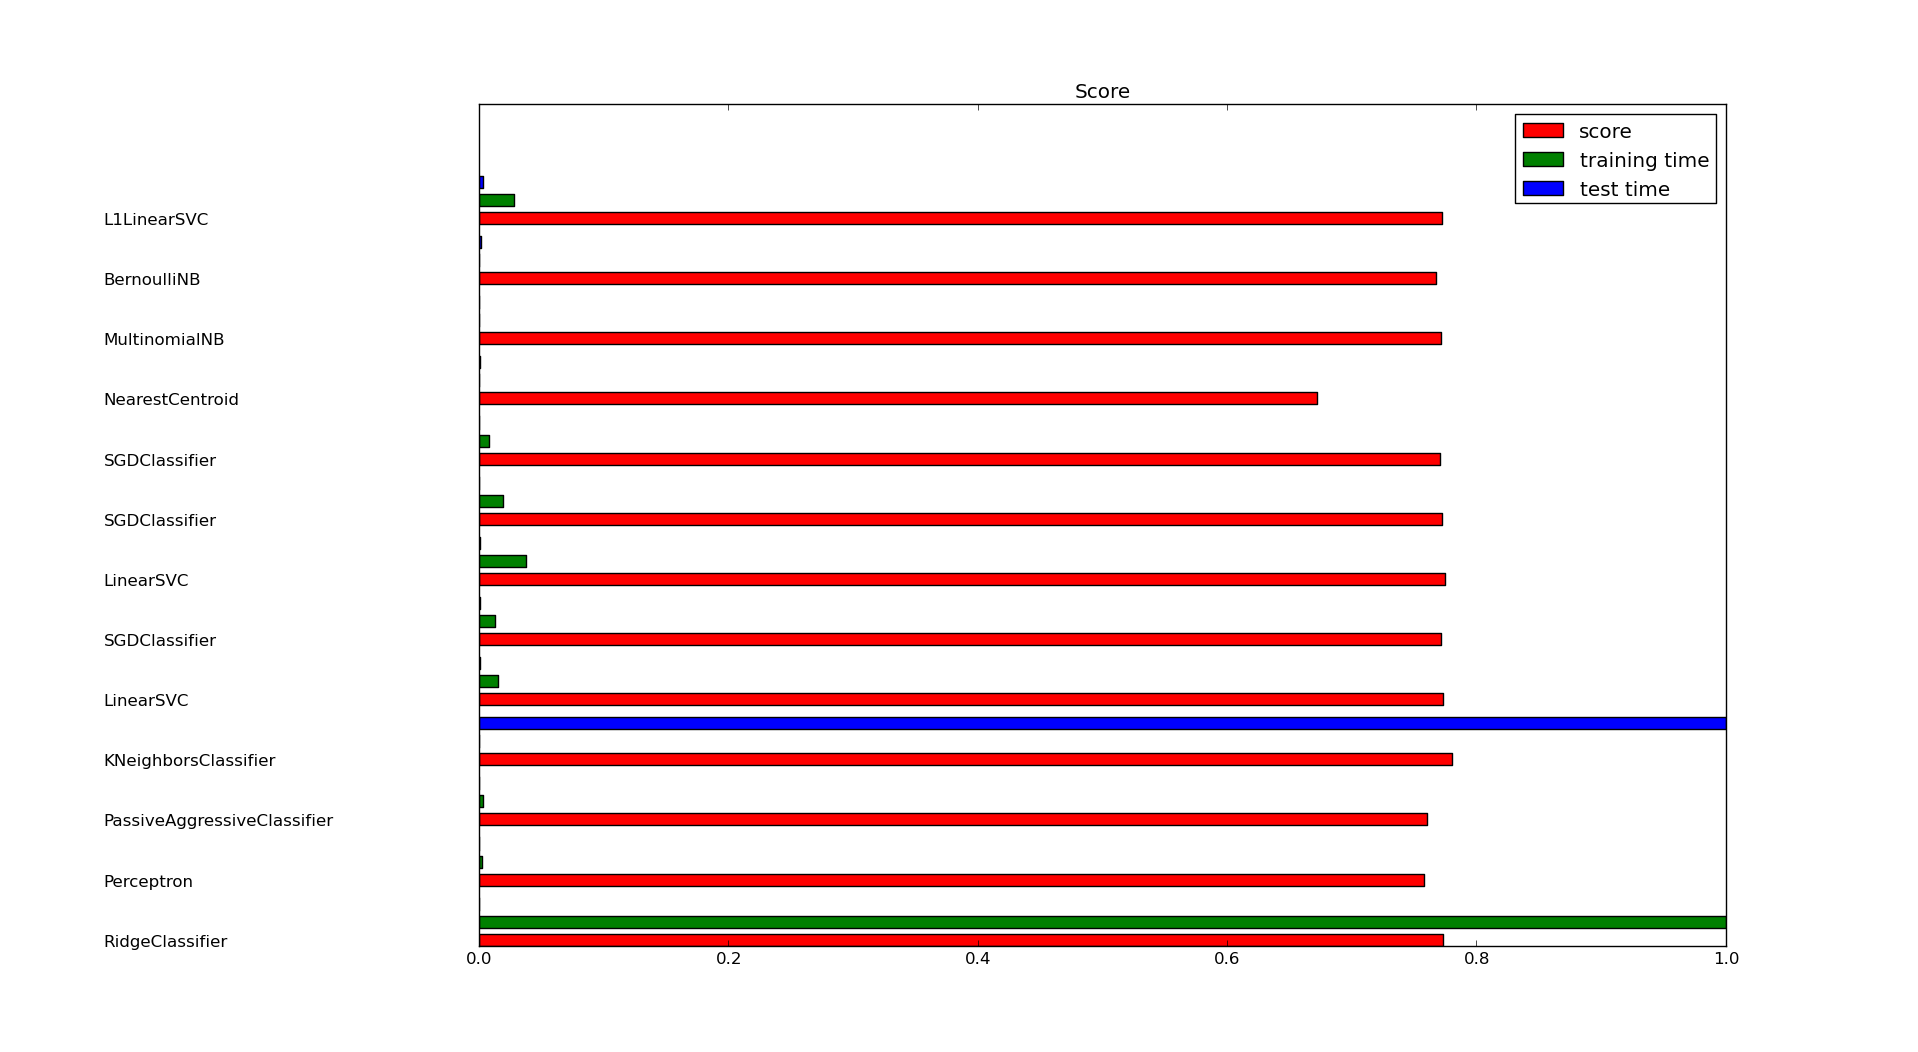
\includegraphics[width=15cm,height=10cm]{figs/scikitlearnclassifierperformance.png}
\caption{Accuracy comparison for different supervised machine learning algorithms and settings generated by classifierselection.py}\label{fig:bugsa}
\end{figure}

\begin{pyverbatim}
 
"""
#Sample of initial results with Naive Bayes and SGDClassifier classifiers
#from classifierselection.py output
"""

================================================================================
Naive Bayes
________________________________________________________________________________
Training: 
MultinomialNB(alpha=0.01, class_prior=None, fit_prior=True)

classification report:
             precision    recall  f1-score   support

      Death       0.00      0.00      0.00         1
        Low       0.51      0.06      0.11       288
   Moderate       0.00      0.00      0.00        93
     NoHarm       0.84      0.99      0.91      2021
     Severe       0.00      0.00      0.00        22

avg / total       0.76      0.83      0.77      2425


________________________________________________________________________________


================================================================================
SGDClassifier
________________________________________________________________________________
Training: 
SGDClassifier(alpha=0.0001, class_weight=None, epsilon=0.1, eta0=0.0,
       fit_intercept=True, l1_ratio=0.15, learning_rate=optimal,
       loss=hinge, n_iter=50, n_jobs=1, penalty=elasticnet, power_t=0.5,
       random_state=None, rho=None, shuffle=False, verbose=0,
       warm_start=False)

classification report:
             precision    recall  f1-score   support

      Death       0.00      0.00      0.00         1
        Low       0.65      0.06      0.11       288
   Moderate       0.00      0.00      0.00        93
     NoHarm       0.84      0.99      0.91      2021
     Severe       0.00      0.00      0.00        22

avg / total       0.78      0.84      0.77      2425


================================================================================


\end{pyverbatim}

\begin{pyverbatim}
#gridsearch.py output

4847 documents
5 categories

Performing grid search...
pipeline: ['vect', 'tfidf', 'clf']
parameters:
{'clf__alpha': (1e-05, 1e-06),
 'clf__n_iter': (10, 50, 80),
 'clf__penalty': ('l2', 'elasticnet'),
 'tfidf__norm': ('l1', 'l2'),
 'tfidf__use_idf': (True, False),
 'vect__max_df': (0.5, 0.75, 1.0),
 'vect__max_features': (None, 5000, 10000, 50000),
 'vect__ngram_range': ((1, 1), (1, 2))}
done in 3681.902s

Best score: 0.842
Best parameters set:
	clf__alpha: 1e-05
	clf__n_iter: 80
	clf__penalty: 'l2'
	tfidf__norm: 'l1'
	tfidf__use_idf: True
	vect__max_df: 1.0
	vect__max_features: None
	vect__ngram_range: (1, 2)
\end{pyverbatim}


\begin{pyverbatim}
#incidenclassify.py output for SGDClassifier with
#gridsearch optimised parameters

 
             precision    recall  f1-score   support

      Death       0.00      0.00      0.00         1
        Low       0.87      0.05      0.09       288
   Moderate       0.00      0.00      0.00        93
     NoHarm       0.84      1.00      0.91      2021
     Severe       0.00      0.00      0.00        22

avg / total       0.80      0.84      0.77      2425

Confusion matrix showing poor performance of 
classification to smaller classes for SGDClassifier

[[                        (predicted)
 [                 Death Low  Mod NoHarm Severe
 [           Death    0    0    0    1    0]
 [           Low      0   13    0  275    0]
 [ (actual)  Moderate 0    1    0   92    0]
 [           NoHarm   0    1    0 2020    0]
 [           Severe   0    0    0   22    0]]


\end{pyverbatim}


